\documentclass[a4paper,14pt]{extarticle}

\usepackage[a4paper,top=20mm,bottom=20mm,left=30mm,right=10mm]{geometry}
\usepackage[T1,T2A]{fontenc}
\usepackage[utf8]{inputenc}
\usepackage[russian]{babel}
\usepackage{indentfirst}
\usepackage{titlesec}
\usepackage{graphicx}
\usepackage{verbatim}
\usepackage{fancyvrb}

\renewcommand{\baselinestretch}{1.3}
\setlength{\parindent}{12.5mm}
\titleformat{\section}{\normalsize\bfseries}{\indent\thesection}{1em}{}
\titleformat{\subsection}{\normalsize\bfseries}{\indent\thesubsection}{1em}{}

\begin{document}

  \newpage\thispagestyle{empty}
  \begin{center}
    \MakeUppercase{
      Министерство науки и высшего образования Российской Федерации\\
      Федеральное государственное бюджетное образовательное учреждение высшего образования\\
      <<Вятский Государственный Университет>>\\
    }
    Институт математики и информационных систем\\
    Факультет автоматики и вычислительной техники\\
    Кафедра электронных вычислительных машин
  \end{center}
  \vfill

  \begin{center}
    \textbf{Работа с графами}\\
    Отчёт по лабораторной работе №4\\
    по дисциплине\\
    <<Дискретная математика>>\\
    Вариант 8
  \end{center}
  \vfill

  \noindent
  \begin{tabular}{ll}
    Выполнил студент гр. ИВТб-1301-05-00 \hspace{5mm} &
    \rule[-1mm]{25mm}{0.10mm}\,/Макаров С.А./\\
    
    Руководитель преподаватель & \rule[-1mm]{25mm}{0.10mm}\,/Пахарева И.В./\\
  \end{tabular}

  \vfill
  \begin{center}
    Киров 2025
  \end{center}

  \newpage
  \section*{\hspace{12.5mm}Цель}
  Цель лабораторной работы: изучение основ теории графов, базовых операций над ними, разработка приложения на языке Паскаль или СИ согласно заданию.

  \section*{\hspace{12.5mm}Задание}
  Неориентированный граф задается матрицей смежности, которая записана в файле. Резмерность: вершин >= 5, дуг >= 7. Сформировать дополнение графа.

  \section*{\hspace{12.5mm}Решение}

  Для решения задач подготовлен ориентированный граф и его дополнение, представленные на рисунке 1.

  \begin{figure}[h]
    \centering
    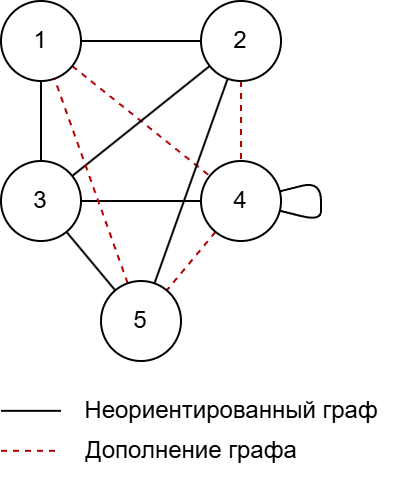
\includegraphics[width=0.4\linewidth]{images/graph.png}
  \end{figure}
  \begin{center}
    Рисунок 1 – Ориентированный граф и его дополнение
  \end{center}

  \pagebreak
  Перед разработкой составлена схема алгоритма, представленная на рисунке 2.

  \begin{figure}[h]
    \centering
    \includegraphics[width=0.99\linewidth]{images/sсheme.png}
  \end{figure}
  \begin{center}
    Рисунок 2 – Схема алгоритма программы
  \end{center}

  \pagebreak
  При разработке реализована программа, исходный код которой представлен ниже.

  \begingroup
    \linespread{1}

    \begin{Verbatim}[tabsize=2]
uses
  SysUtils;

var
  matrix: array [1..5, 1..5] of integer;
  i, j, k: integer;
  fileInput: text;
  fileLine: string;

begin
  assign(fileInput, 'input.txt');
  reset(fileInput);
  writeln('Матрица смежности', #10);

  write('  ');
  for i := 1 to 5 do
    write(' ', i, ' ');
  writeln();

  i := 1;

  while not Eof(fileInput) do
  begin
    write(i, '  ');
    readln(fileInput, fileLine);
    j := 1;

    for k := 1 to Length(fileLine) do
    begin
      if fileLine[k] <> ' ' then
      begin
        if (fileLine[k] = '1') or (i = j) then
          matrix[i][j] := 0
        else
          matrix[i][j] := 1;

        write(fileLine[k], '  ');
        j := j + 1;
      end;
    end;
    writeln();

    i := i + 1;
  end;
  writeln();

  writeln('Дополнение графа', #10);

  write('  ');
  for i := 1 to 5 do
    write(' ', i, ' ');
  writeln();

  for i := 1 to 5 do
  begin
    write(i, '  ');
    for j := 1 to 5 do
      write(matrix[i][j], '  ');
    writeln();
  end;

  readln;
end.
    \end{Verbatim}
  \endgroup

  Экранная форма программы в виде консольного приложения представлена на рисунке 3.

  \begin{figure}[h]
    \centering
    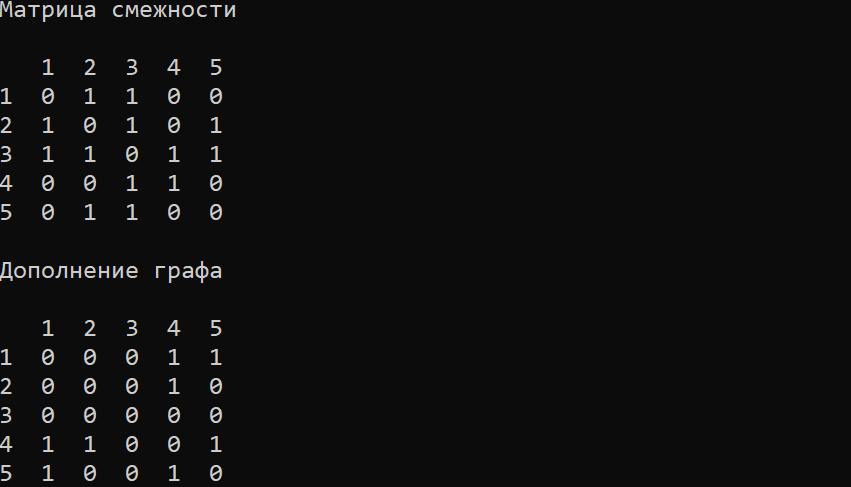
\includegraphics[width=0.8\linewidth]{images/image.png}
  \end{figure}
  \begin{center}
    Рисунок 3 – Консольный интерфейс программы
  \end{center}

  \section*{\hspace{12.5mm}Вывод}
  В процессе выполнения лабораторной работы, при решении предложенных задач, реализована программа на языке Паскаль, которая выполняют такую операцию, как дополнение графа для матрицы смежности, заданной в файле.

\end{document}